\documentclass{beamer}
\usepackage{graphicx}
\usepackage{hyperref}
\usepackage{tikz}
\usetheme{Madrid}
\definecolor{ginger}{rgb}{0.69, 0.4, 0.0}
\usecolortheme{beaver}
\titlegraphic{
\includegraphics[width=2.5cm]{logo.png}
}
\title[Interaction of Laser with Plasma]{Interaction of Relativistic and non-Relativistic Laser Pulse With Plasma}
\date{}
\institute[IIT Delhi]{\large Indian Institute of Technology, Delhi}
\author[]{Kulwinder Kaur (2021PHS7190)\\ Harikesh Kushwaha (2021PHS7181)\\[3mm]Adviser: Prof. Vikrant Saxena}
\vspace{0cm}
\begin{document}
\maketitle
\begin{frame}{Introduction}
    \frametitle{Introduction}
    \small
    \begin{itemize}
        \item Plasma is a quasineutral gas of charged and nuetral particles which exhibits collective behaviour.
        \item If an electron in plasma is displaced from its equilibrium position, it will start oscillating around its equilibrium position. The frequency of oscillation is characteristics of the plasma parameters and is called plasma frequency.
        \item A plasma is underdense for an electromagnetic wave if its frequency is less than the frequency of the em wave. On the other hand, a plasma is overdense if its frequency is greater than the frequency of the em wave.
        \item The simulation uses \textit{EPOCH}, a parallised, second order and fully relativistic implementation of particle in cell
              (PIC) algorithm.
        \item Non-relativistic as well as relativistic laser pulses are used to study the interaction of laser with plasma.
    \end{itemize}
\end{frame}
\begin{frame}
    \small
    \frametitle{PIC Algorithm}
    Particle in Cell (PIC) is a numerical approach that simulates a collection of particles that interact via external and self-induced electromagnetic fields.
    \begin{itemize}
        \item Replace a system of charges with a macro particle having the same charge to mass ratio.
        \item Decretise the space by drawing line parallel to the boundaries of the system.
        \item Replace the continuous electric and magnetic by values on the descete mesh.
        \item Interpolate the charge on the grid to update the fields.
        \item Update $\mathbf{E}$ from step $n$ to $n+1$ is done via central differencing using $\mathbf{B}$ at $n+1/2$.
        \item Update $\mathbf{B}$ from step $n-1/2$ to $n+1/2$ is done via central differencing using $\mathbf{E}$ and the current density ($\textbf{J}$) at step $n$.
        \item The updated electric and magnetic fields are used to forward velocity for step $n-1/2$ to $n+1/2$
    \end{itemize}
\end{frame}
\begin{frame}
    \small
    \begin{itemize}
        \item Velocity at step $n+1/2$ is used to forward position for step $n$ to $n+1$.
    \end{itemize}
    \begin{figure}
        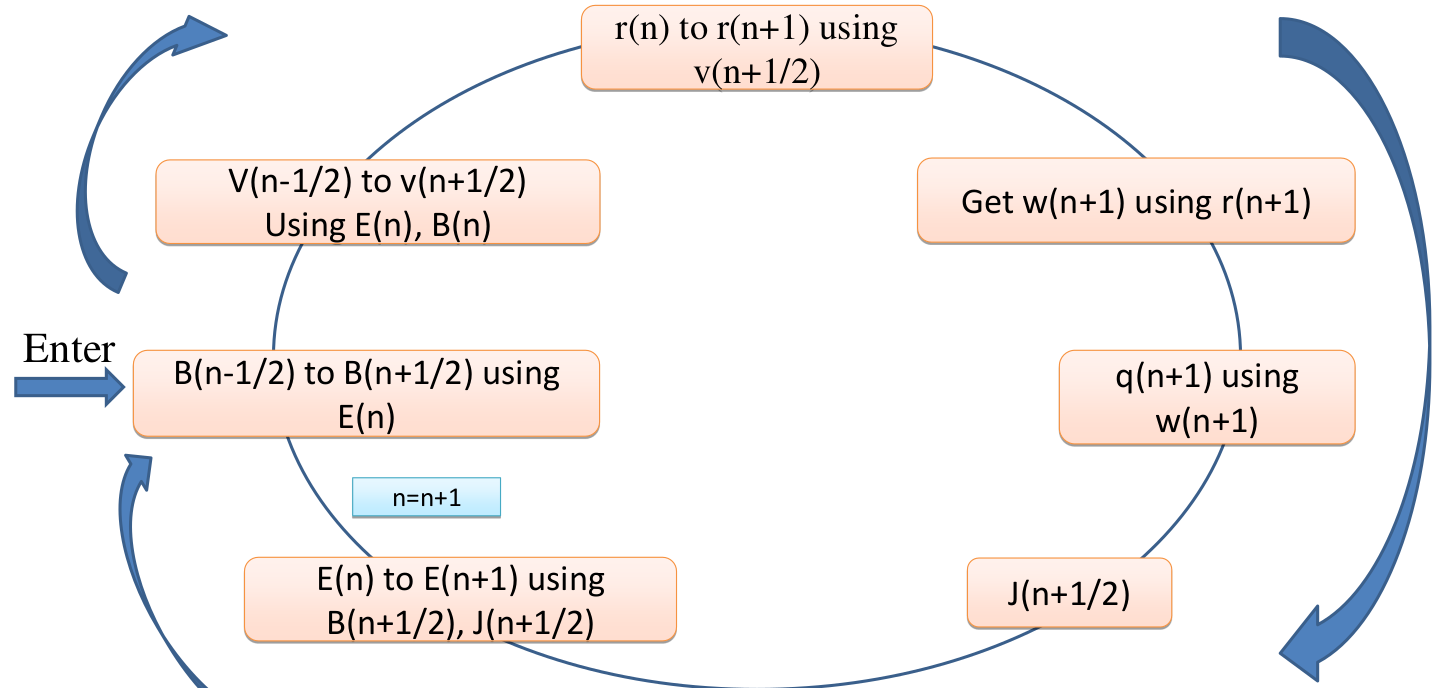
\includegraphics[width=10cm, height=7cm]{PIC.png}
        \centering
        \caption{The PIC Cycle}
    \end{figure}
\end{frame}
\begin{frame}
    \small
    \frametitle{Simulation Parameters}
    For a laser of frequency $\omega_l$ and electric field amplitude $E_0$, the laser vector potential is defined as
    $
        a_0 = \frac{eE_0}{m w_l c}
    $
    . A laser is called relativistic if $a_0 \ge 1$.
    \begin{itemize}
        \item The simulation box extends for $20 \lambda _l$ (from $-10 \lambda _l$ to $10 \lambda _l$), where $\lambda_l$ is the laser wavelength and has total 1000 cells.
        \item  The plasma is placed at $x=0$ and with a thickess of $\lambda_l$.
        \item  Number of particles per cell are 100.
        \item The plasma density $n_p$ is defined in terms of the critical density $n_c$ and is varied from 0.1 to 10.
        \item The vector potential $a_0$ is used as 0.1, 1.0 and 10.0.
    \end{itemize}
    The envelope of the incident laser field varies according to
    % \tiny
    \begin{equation}
        P(t)=
        \begin{cases}
             & \sin^2(\pi t/T) \text{ for } 0 \leq t \le T \\
             & 0         \;      \text{ otherwise }
        \end{cases}
    \end{equation}
    Where T is the pulse duration here taken as $T=10\tau$ with $\tau = 2\pi/\omega_l$ is the time of one laser cycle. The simulation is performed for $t=20\tau$.
\end{frame}
\begin{frame}
    \frametitle{Result and Discussion}
    \small
    \begin{columns}
        \begin{column}{0.3\textwidth}
            We define a term
            $
                R= \frac{{E_{300}^2}-{E_{600}^2}}{{E_{300}^2}}
            $\\
            The plot of R with different ratio of $n_c$ and $n_0$ is shown in the figure 1 for different values of vector potential $a_0$. We find a shifting of the critical density for relativistic laser pulse.
        \end{column}
        \begin{column}{0.7\textwidth}  %%<--- here
            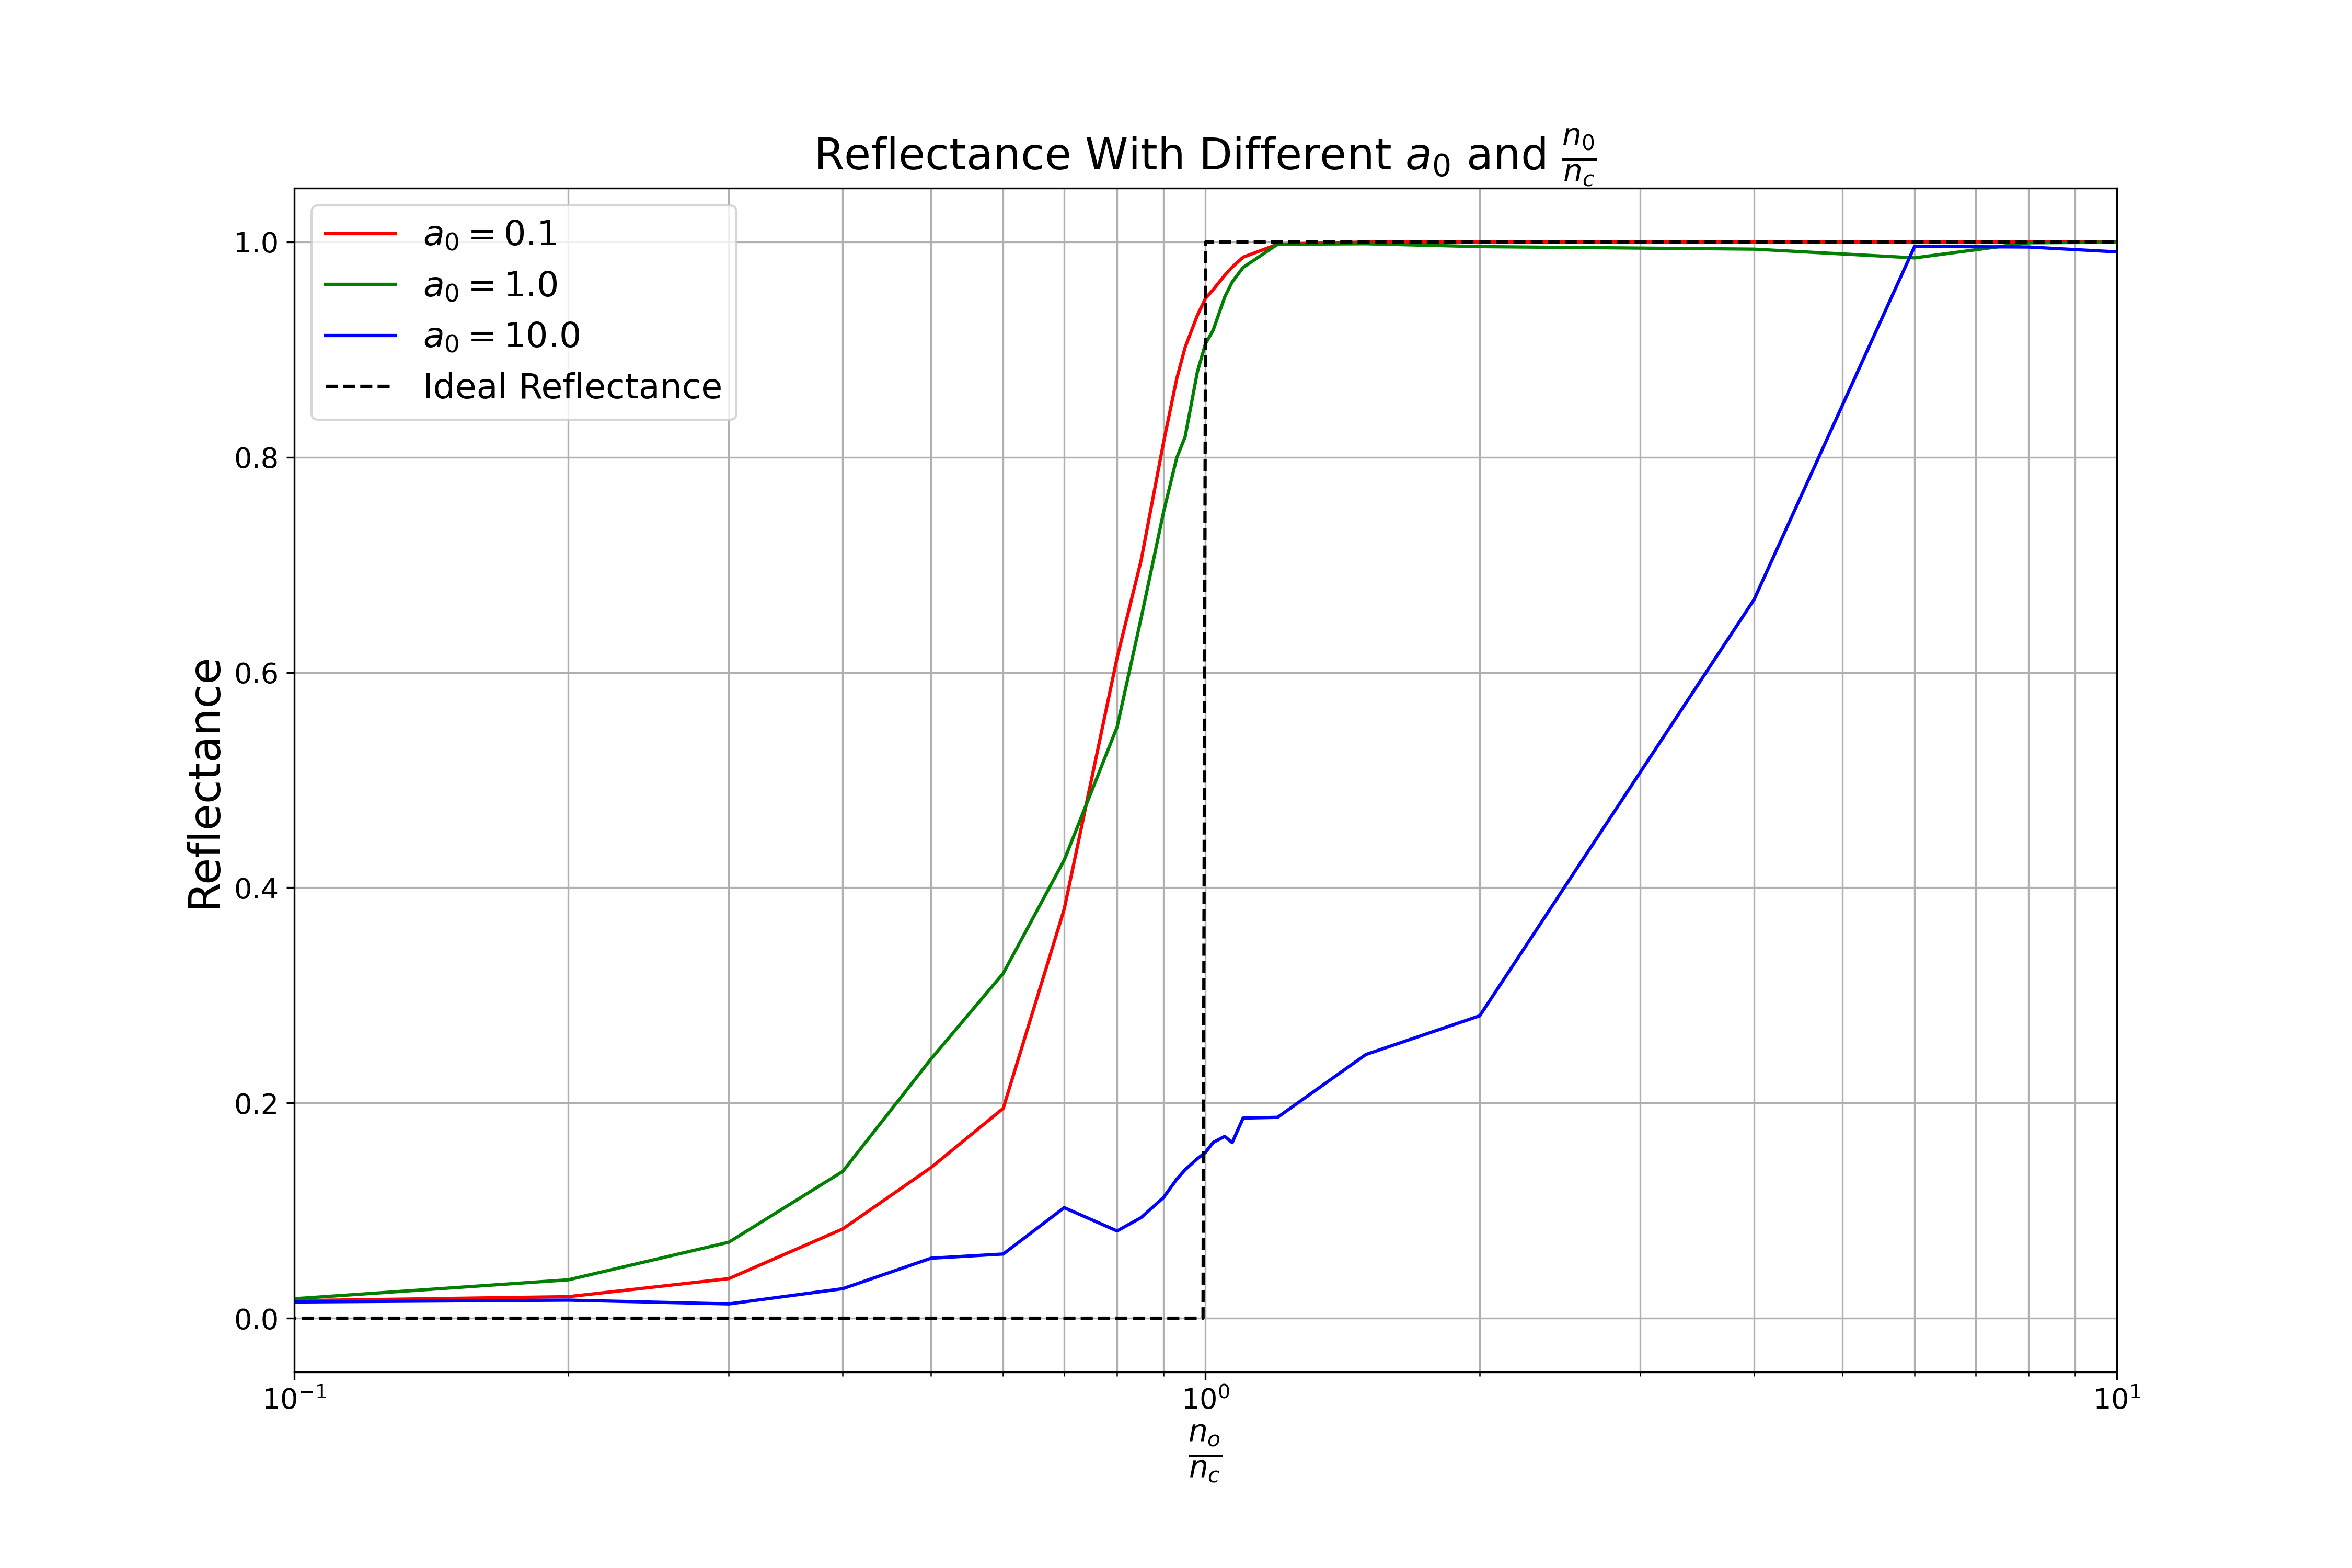
\includegraphics[width=8cm, height=6cm]{reflection.png}
            % \centering
            % \caption{The PIC Cycle}
        \end{column}
    \end{columns}
\end{frame}
\begin{frame}
    \small
    \begin{columns}
        \begin{column}{0.3\textwidth}
            The electron density with time is plotted for different $a_0$. The plot shows that the oscillation of electrons increases with increasing vector potential.
        \end{column}
        \begin{column}{0.7\textwidth}  %%<--- here
            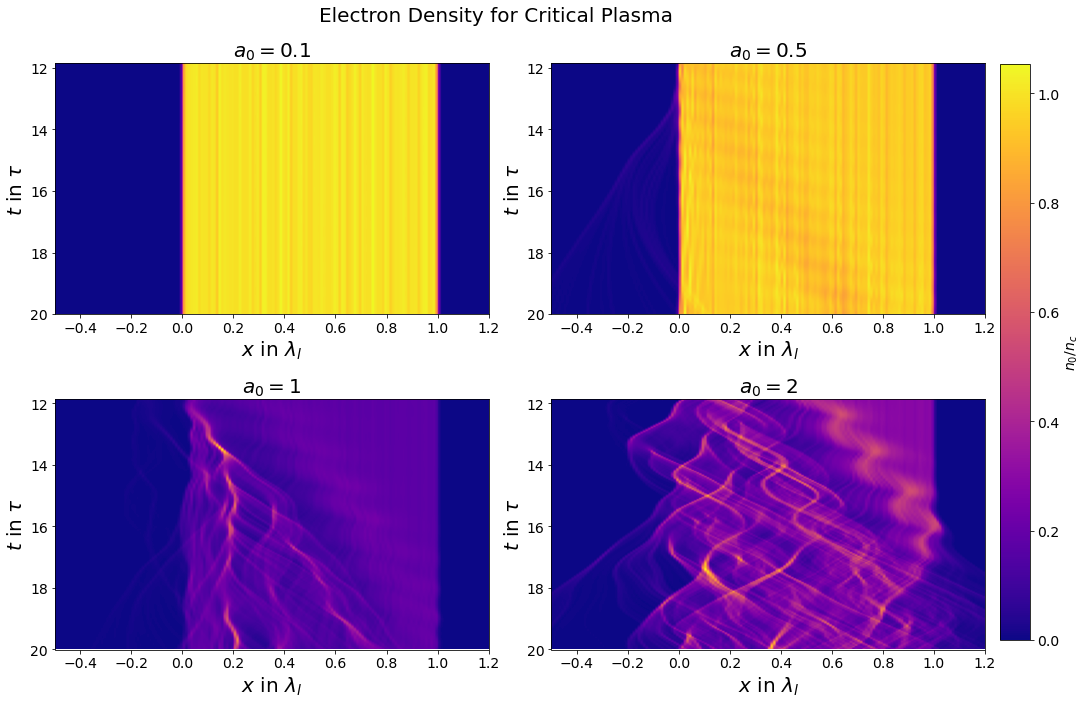
\includegraphics[width=8cm, height=6cm]{density.png}
            % \centering
            % \caption{The PIC Cycle}
        \end{column}
    \end{columns}
\end{frame}
\begin{frame}
    \frametitle{Conclusion}
    \small
    \begin{itemize}
        \item When the laser becomes relativistic for $a_0 \ge 1$, the particles inside plasma starts to oscillate with relativistic velocity, gaining mass. This results in change in the plasma frequency and hence the laser does not get reflected even for density greater than the critical density corresponding to the non-relativistic case.
        \item The laser pulse, after interacting with electrons, makes them oscillate. If the pulse becomes relativistic, the oscillations becomes strong and hence the plasma surface oscillates with relativistic velocity.
    \end{itemize}
    \section{References}

    \begin{thebibliography}{9}
        \bibitem{lichters}
        R. Lichters Et al. Physics of Plasmas 3, pp. 3425-3437 (1996)

        \bibitem{epoch}
        Arber, T D Et al. Plasma Physics and Controlled Fusion 57 1-26 (2015)

        \bibitem{suciu}
        Alin Suciu Et al. 2020 15th Conference on Computer Science and Information Systems (FedCSIS), pp.381-385, 2020

        \bibitem{chen}
        Francis F. Chen
        Introduction to Plasma Physics and Controlled Fusion $3^{rd}$ Ed.

    \end{thebibliography}
\end{frame}
\end{document}